% questions.tex —— 1977 年·江苏卷 · 题目内容片段（无答案）
% 由 tools/generate_projects.py 依来源总账自 1977/1977_数学真题_江苏_试题.md 生成，勿手改（改源 MD 后重跑）


\gkpart{数学试卷（江苏卷）}

\begin{gktip}
\textbf{来源说明}：本题面依据固定源 PDF《1977 年普通高等学校招生考试（江苏卷）数学试卷》单页扫描逐题转录。源文件为 A3 单页题面，正式题为第 1—6 题，题面中“附加题”栏的第 7、8 题不计入正式题量。第 1(1) 的负数半次幂和附加题 7 的极限变量/被开方变量均按源页原样保留，相关疑点见答案要点与解析正文。
\end{gktip}

\begin{question}
\gkti{1}解答下列各题：

\Needspace{5\baselineskip}
（1） 计算：

\nopagebreak[4]
\[
\left(2\frac14\right)^{\frac12}+\left(\frac1{10}\right)^{-2}-(3.14)^0+\left(-\frac{27}{8}\right)^{-\frac12}
\]

\Needspace{5\baselineskip}
（2） 求函数

\nopagebreak[4]
\[
y=\sqrt{x-2}+\frac1{x-3}+\lg(5-x)
\]

的定义域。

\Needspace{5\baselineskip}
（3） 解方程：

\nopagebreak[4]
\[
5^{x^2+2x}=125
\]

\Needspace{5\baselineskip}
（4） 计算：

\nopagebreak[4]
\[
-\log_3\left(\log_3\sqrt[3]{\sqrt[3]{\sqrt[3]{3}}}\right)
\]

\Needspace{5\baselineskip}
（5） 把直角坐标方程

\nopagebreak[4]
\[
(x-3)^2+y^2=9
\]

化为极坐标方程。

\Needspace{5\baselineskip}
（6） 计算：

\nopagebreak[4]
\[
\lim_{n\to\infty}\frac{1+2+3+\cdots+n}{n^2}
\]

\Needspace{5\baselineskip}
（7） 分解因式：

\nopagebreak[4]
\[
x^4-2x^2y-3y^2+8y-4
\]

\end{question}
\begin{question}
\gkti{2}过抛物线 $y^2=4x$ 的焦点作倾斜角为 $\dfrac{3\pi}{4}$ 的直线，它与抛物线相交于 $A\text{、}B$ 两点。求 $A\text{、}B$ 两点间的距离。

\Needspace{0.4\textheight}
\end{question}
\begin{question}
\gkti{3}在直角三角形 $ABC$ 中，$\angle ACB=90^\circ$，$CD\text{、}CE$ 分别为斜边 $AB$ 上的高和中线，且 $\angle BCD$ 与 $\angle ACD$ 之比为 $3:1$，求证：$CD=DE$。
\nopagebreak[4]
\begin{center}% 1977 年江苏卷第 3 题：直角三角形中的高与中线
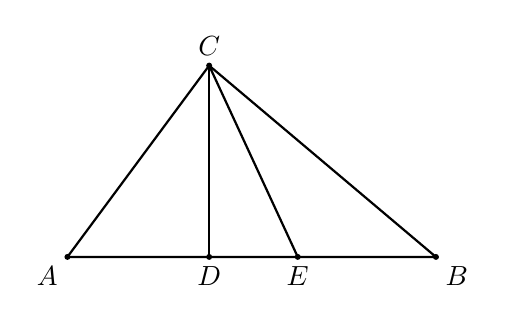
\begin{tikzpicture}[scale=0.9]
  \coordinate (A) at (0,0);
  \coordinate (D) at (2.0,0);
  \coordinate (E) at (3.25,0);
  \coordinate (B) at (5.2,0);
  \coordinate (C) at (2.0,2.7);
  \draw[thick] (A)--(C)--(B)--cycle;
  \draw[thick] (C)--(D);
  \draw[thick] (C)--(E);
  \fill (A) circle (1.2pt) node[below left] {$A$};
  \fill (B) circle (1.2pt) node[below right] {$B$};
  \fill (C) circle (1.2pt) node[above] {$C$};
  \fill (D) circle (1.2pt) node[below] {$D$};
  \fill (E) circle (1.2pt) node[below] {$E$};
\end{tikzpicture}
\end{center}
\nopagebreak[4]
\end{question}
\begin{question}
\gkti{4}在周长为 $300\ \mathrm{cm}$ 的圆周上，有甲、乙两球以大小不等的速度作匀速圆周运动。甲球从 $A$ 点出发按逆时针方向运动，乙球从 $B$ 点出发按顺时针方向运动，两球相遇于 $C$ 点；相遇后，两球各自反方向作匀速圆周运动，但这时甲球速度的大小是原来的 2 倍，乙球速度的大小是原来的一半，以后他们第二次相遇于 $D$ 点。已知弧 $\overset{\frown}{AmC}=40\ \mathrm{cm}$，弧 $\overset{\frown}{BnD}=20\ \mathrm{cm}$，求弧 $\overset{\frown}{ACB}$ 的长度。

\end{question}
\begin{question}
\gkti{5}

（1） 若三角形三内角成等差数列，求证：必有一内角为 $60^\circ$。

（2） 若三角形三内角成等差数列，而且三边又成等比数列，求证：三角形三内角都是 $60^\circ$。

\end{question}
\begin{question}
\gkti{6}在两条平行直线 $AB$ 和 $CD$ 上分别取定一点 $M$ 和 $N$，在线段 $AB$ 上取一定线段 $ME=a$；在线段 $MN$ 上取一点 $K$，连结 $EK$ 并延长交 $CD$ 于 $F$。试问 $K$ 取在哪里时，$\triangle EMK$ 与 $\triangle FNK$ 的面积之和最小？最小值是多少？

\begin{gktip}
\Needspace{0.25\textheight}
\textbf{附加题}
\end{gktip}

\Needspace{5\baselineskip}
\textbf{附加题 7．} 求极限：

\nopagebreak[4]
\[
\lim_{n\to\infty}\sqrt{x}\left(\sqrt{x+1}-\sqrt{x}\right)
\]

\Needspace{5\baselineskip}
\textbf{附加题 8．} 求不定积分：

\nopagebreak[4]
\[
\int\frac{\mathrm dx}{(1+\mathrm e^x)^2}
\]

\end{question}